\documentclass{vskpou} % Nacteni tridy

\usepackage[utf8]{inputenc}
\usepackage{graphicx}
\graphicspath{{images/}}
\usepackage{fancyhdr}

\usepackage{natbib}
\pagestyle{fancy}

\usepackage[IL2]{fontenc}        

\jazyky{czech}{english}

\hlavnijazyk{czech}








%% Zde zadejte resume
\resume{Tato semestrální práce je zaměřena na vývoj mobilních aplikací pomocí jazyků Java a Kotlin. Za tímto účelem byla vytvořena mobilní aplikace, která slouží jako manuál pro tvorbu aplikací pro Android OS. Nejprve bylo zapotřebí charakterizovat celý operační systém a jeho jednotlivé vrstvy. Poté programovací jazyky a nástroje, které slouží pro vývoj aplikací. V závěru je vysvětlen způsob testování aplikací a jejich následné publikování.}{This semester's thesis is focused on the development of mobile applications using Java and Kotlin. To this end, a mobile application was created, which serves as a manual for creating applications for Android OS. First it was necessary to characterize the entire operating system and its individual layers. Then the programming languages and tools that serve as application development. In the end, the method of testing applications and then publishing them is explained.}




%
\begin{titlepage}
\begin{center}

\Large{OSTRAVSKÁ UNIVERZITA} \\
\Large{PŘÍRODOVĚDECKÁ FAKULTA}\\
\Large{KATEDRA INFORMATIKY A POČÍTAČŮ}
\vspace{8cm}

\huge{\textbf{Tvorba mobilní aplikace}}\\
\vspace{1cm}
\Large{SEMESTRÁLNÍ PRÁCE}

\vspace{7cm}

\end{center}

\normalsize{Autor: Jan Sonnek \hfill Ostrava, 2021}

\end{titlepage}



\begin{titlepage}
\begin{center}

\Large{OSTRAVSKÁ UNIVERZITA} \\
\Large{PŘÍRODOVĚDECKÁ FAKULTA}\\
\Large{KATEDRA INFORMATIKY A POČÍTAČŮ}
\vspace{8cm}

\huge{\textbf{Tvorba mobilní aplikace}}\\
\vspace{1cm}
\Large{SEMESTRÁLNÍ PRÁCE}

\vspace{7cm}

\end{center}

\normalsize{Autor: Jan Sonnek \hfill Ostrava, 2021}

\end{titlepage}


\begin{document}
\thispagestyle{empty}
\setcounter{page}{1}

\clearpage
%%%%%%%%%%%%%%%%%%%%%%%%%%%%%%%%%%%%%%%%%%%%%%%%%%%%%%%%%%%%%%%%%%%%%%%%%
\section{ANDROID}
Android je operační systém, který vytvořila společnost Google. Na rozdíl od hlavního konkurenta Applu, je Android open-source, což znamená otevřený operační systém se zdrojovým kódem. Každý vývojář jej může používat a upravovat dle vlastních představ, ačkoliv musí dodržovat určitá pravidla. OS je založen na linuxovém jádře různých verzí, které zajišťuje zabezpečení systému jako celku, správu paměti, správu procesů, přístup k síti a ovladačům všech vnitřních senzorů a komponentů. Android je nejmladší a nejrychleji se rozvíjející multiplatformní operační systém primárně vyvíjen jako platforma převážně pro PDA, chytré mobily (smartphony) a tablety. Kromě zmíněných zařízení se s ním setkáme v chytrých hodinkách (smartwatch), televizích (Android TV) nebo v autě (Android Auto).\cite{10} \\
\\
Jak již bylo zmíněno, Android je multiplatformní OS, což znamená, že systém může běžet na zařízeních různých značek (Samsung, Lenovo, Huawei, Honor, atd). Podpora několika značek má i své nevýhody. Mezi největší nevýhodou je optimalizace systému na konkrétní určitou platformu (aktualizace nové verze Androidu).  V optimalizaci systému vítězí Apple iOS. Proto, když se zeptáte lidí, proč preferují iOS než Android OS, bývá jejich odpověď většinou právě okamžitá aktualizace OS.\cite{10} 

\subsection{Historie OS}
I když OS patří společnosti Google, za jejím vznikem nestojí. Jejím zakladatelem je společnost Android Inc., která vznikla v říjnu roku 2003 ve městě Palo Alto, ve státě Kalifornia. O dva roky později Google odkoupil Android Inc. Odhadovaná částka, kterou Google za Android zaplatil činí 50 milionů dolarů. V listopadu 2007 byla založena Open Handset Aliance, která stojí za vývojem Androidu dodnes. Open Handset Aliance je sdružení více než 80 firem, mezi které patří Intel, HTC, LG, NVIDIA, Qualcomm, Google nebo Samsung, a to v oblasti mobilních operátorů, softwarových společností, společností vyrábějících polovodičové součástky nebo výrobci mobilních zařízení. V té době také vychází vývojářský Kit (SDK). V září 2008 se na trhu v USA objevil mobil HTC Dream (G1) s Androidem 1.0. V únoru 2009 přišel Android 1.1 jako aktualizace pro G1. V dubnu 2009 spatřil světlo světla první masový Android s verzí 1.5 (Cupcak). Odstartoval tak popularitu tohoto systému.\cite{10} 
\newpage
\begin{figure}[h!]
\centering
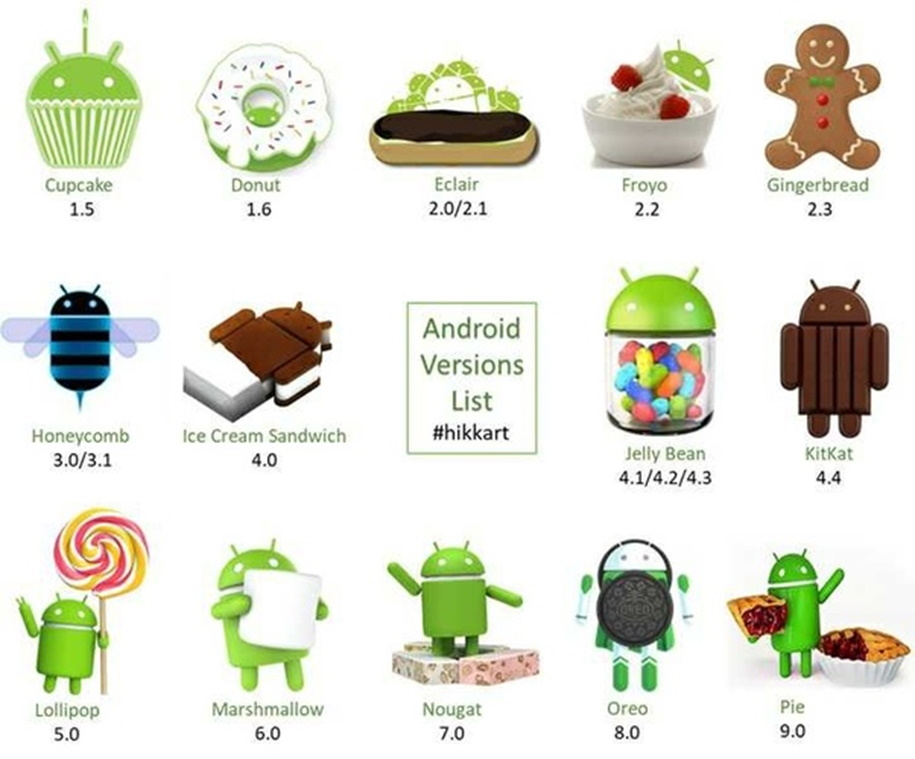
\includegraphics[scale=0.5]{images/1.jpg}
\caption{Loga verzí OS}
\label{1}
\end{figure}
\clearpage




\begin{center}

\begin{tabular}{ |p{3cm}|p{3cm}|p{3cm}|p{3cm}| }

\hline
\multicolumn{4}{|c|}{Přehled verzí Android} \\
\hline
Název& Verze &Rok vydání&API \\
\hline
Android Apple Pie & 1.0 & 2008 & 1\\
\hline
Android Banana Bread &
1.1&
2009&
2\\
\hline
Android Cupcake&
1.5&
2009&
3 \\
\hline
Android Donut&
1.6&
2009&
4\\
\hline
Android Eclair&
2.0&
2009&
5 \\
\hline
Android Eclair&
2.0.1&
2009&
6 \\
\hline
Android Eclair&
2.1&
2010&
7 \\
\hline
Android Froyo&
2.2, 2.2.1 – 2.2.3&
2010&
8 \\

\hline
Android Gingerbread&
2.3, 2.3.1&
2010&
9 \\
\hline
Android GIngerbread&
2.3.2 – 2.3.7&
2011&
10 \\
\hline
Android Honeycomb&
3.0, 3.1, 3.2&
2011&
11 \\
\hline
Android Honeycomb&
3.2.1, 3.2.2, 3.2.3&
2011&
12 \\
\hline
Android Honeycomb&
3.2.6&
2012&
13 \\
\hline
Android Ice Cream Sandwich&
4.0&
2011&
14 \\
\hline
Android Ice Cream Sandwich&
4.0.1, 4.0.2, 4.0.3, 4.0.4&
2012&
15 \\
\hline
Android Jelly Bean&
4.1&
2012&
16 \\
\hline
Android Jelly Bean&
4.1.1, 4.1.2&
2012&
17 \\
\hline
Android Jelly Bean&
4.2, 4.2.1 , 4.2.2&
2013&
18 \\
\hline
Android KitKat&
4.4&
2013&
19 \\
\hline





\end{tabular}

\end{center}







\begin{center}
\begin{table}[h]
\begin{tabular}{ |p{3cm}|p{3cm}|p{3cm}|p{3cm}| }



\hline
Android Kitkat&
4.4W2&
2014&
20 \\
\hline
Android Lollipop&
5.0&
2014&
21 \\
\hline
Android Lollipop&
5.1.1&
2015&
22 \\
\hline
Android Marshmallow&
6.0&
2015&
23 \\
\hline
Android Nougat&
7.0&
2016&
24 \\
\hline
Android Nougat&
7.1.1&
2016&
25 \\
\hline
Android Oreo&
8.0&
2017&
26 \\
\hline
Android Oreo&
8.1&
2017&
27 \\
\hline
Android Pie&
9.0&
2018&
28 \\
\hline
Android 10&
10.0&
2019&
29 \\
\hline




\end{tabular}
\caption{Vlastní tvorba verzí OS Android}
\end{table}
\end{center}





\newpage
\subsection{Architektura Androidu}
Celá architektura operačního systému se skládá z pěti vrstev, které jsou znázorněny na obrázku č.~\ref{1}.

\begin{figure}[h!]
\centering
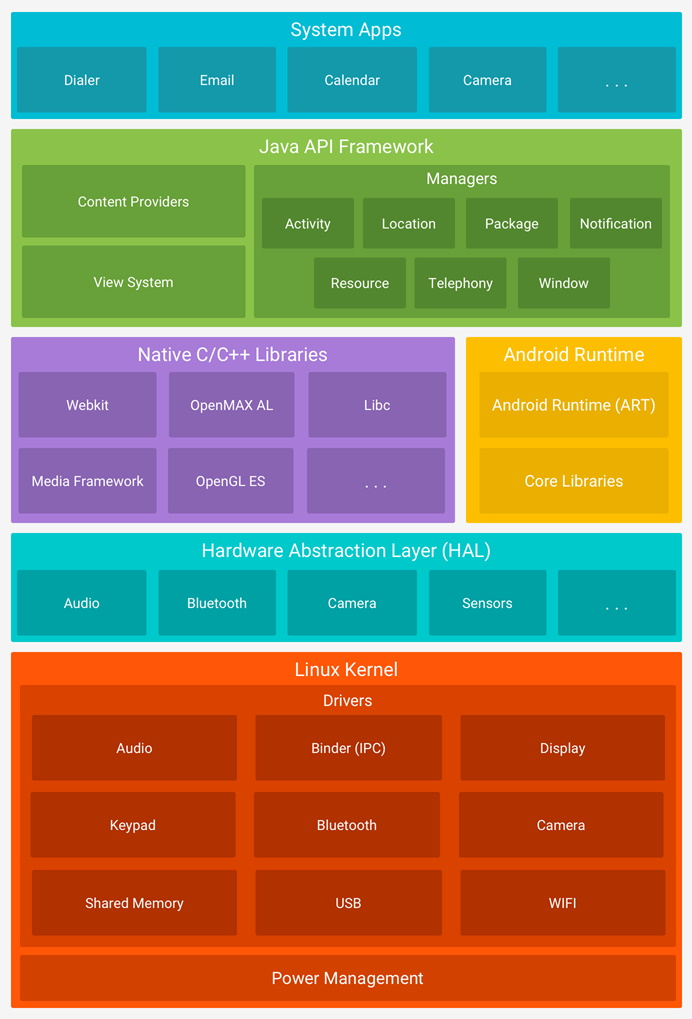
\includegraphics[scale=0.5]{images/2.jpg}
\caption{Architektura OS Android}
\label{1}
\end{figure}

\begin{itemize}
    \item Linux Kernel
    \item Hardware Abstraction Layer
    \item Nativní knihovny (NDK)
    \item Android Runtime – ART
    \item Java API Framework
\end{itemize}
\newpage
\subsubsection{Linux Kernel}
Na nejnižší vrstvě Androidu se nachází jádro neboli Linux Kernel a patří mezi nejzákladnější komponenty systému Android. \uv{\,\textit{Základní funkcí je implementace abstrakce mezi použitým hardwarem a softwarem ve vyšších vrstvách. Zabezpečuje správu paměti, správu procesů, základní síťovou vrstvou a ovladače. Řízení procesů umožňuje, aby více procesů běželo současně, aniž by se vzájemně ovlivňovaly.}}\footnote{Mistrovství - Android. Brno: Computer Press, 2017. ISBN 978-80-251-4875-4.}\textit{Mistrovství Android -- str. 75}\cite{10}
\subsubsection{Hardware Abstraction Layer}
Vzhledem k odchylnosti hardwarových zařízení mobilních telefonů či tabletů, jako je např. procesor nebo fotoaparát, na nichž může Android běžet, byla vytvořena vrstva Hardware Abstraction Layer (vrstva abstrahující hardware), zkráceně HAL. HAL vrstva se nachází nad úrovní Linux Kernel a vytváří rozhraní pro komunikaci s vyššími vrstvami systému s hardwarem. Z vývojářského hlediska je HAL dobrý v tom, že programátor nemusí přesně znát hardwarové specifikace všech možných zařízení.\cite{10},\cite{17}


\begin{figure}[h!]
\centering
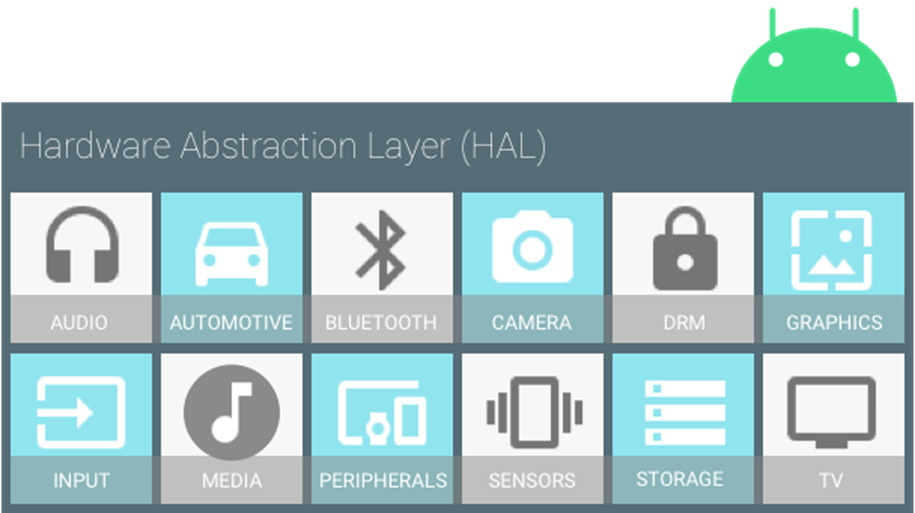
\includegraphics[scale=0.5]{images/3.jpg}
\caption{HAL}
\label{3}
\end{figure}

\subsubsection{Nativní knihovny}
Jednou z dalších vrstev Androidu jsou nativní knihovny (NDK). Tvoří mezivrstvu mezi různými komponenty vyšších vrstev a linuxovým jádrem. NDK jsou napsané v C/C++. Při programování může vývojář použít již existující knihovny nebo si knihovnu jednoduše naprogramovat dle potřeby sám. Webkit, který je součástí NDK, je určen k renderování a zobrazení webových stránek. Na této úrovni jsou implementovány také knihovny médií a grafické 2D. Pro vykreslování 3D grafiky slouží knihovna OpenGL založená na OpenGL ES (OpenGLforEmbedded Systems). Systémová knihovna LibC je knihovna optimalizovaná pro mobilní zařízení, která obsahuje jen části, které jsou zapotřebí pro Android.\cite{10},\cite{17} 

\subsubsection{Android Runtime - ART}
Aplikace pro Android, které jsou vytvořeny v Android Studio jsou sestaveny do bajtového mezikódu, označovaného DEX. Soubory DEX vznikly kompilací z klasických souborů CLASS (soubory, ve kterých se píše zdrojový kód v jazyku Java nebo Kotlin) a JAR (vytvořená Java aplikace). Jsou kompaktnější než klasické soubory CLASS. Když se následně aplikace načítá do zařízení, Android Runtime (ART) používá proces označovaný jako Ahead-Of-Time (AOT) Tento proces se používá na přeložení bajtového kódu do nativních instrukcí konkrétního procesoru v příslušném zařízení. Jednoduše řečeno, ART slouží pro přeložení zdrojového kódu do strojového kódu (1 a 0).\cite{10},\cite{17} 

\subsubsection{Java API Framework}
Aplikační framework obsahuje v aplikacích opakovaně použitelný software, mezi které patří např. ovládací prvky, ikony atd. Tento framework je napsán v programovacím jazyku Java a je to nejdůležitější vrstva pro vývojáře mobilních aplikací. Poskytuje aplikacím základní služby systému. Celý Java API Framework se skládá z:\cite{17}



\begin{itemize}
    \item Package Manager - 
    Můžeme si package manager představit jako databázi. Tato databáze (package manager) má za úkol udržet všechny aktuální aplikace, které jsou na daném zařízení nainstalovány. Grafickým znázorněním package manageru není nic jiného než obrazovka zařízení, kde je možné vidět všechny nainstalované aplikace (Chrome, Obchod Play, YouTube, Gmail, Google, Disk, Fotky atd). Každá tato aplikace má svoji jedinečnou ikonu, která reprezentuje balíček aplikace.\cite{17}
    
    \item Windows Manager - Windows Manager má na starosti správu oken, které tvoří mobilní aplikace. Aplikace většinou využívají dvě a více oken současně.
    \begin{figure}[h!]
\centering
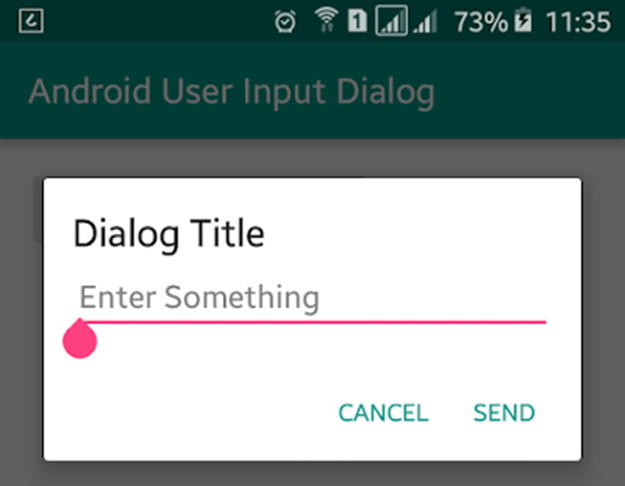
\includegraphics[scale=0.5]{images/4.jpg}
\caption{Windows Manager}
\label{4}
\end{figure}

Na obrázku \ref{4} můžete vidět několik oken. Nejdůležitější je hlavní okno aplikace (Android User Input Dialog) a dialogové okno. Z obrázku můžeme tedy vidět, že aplikace má otevřené dvě okna současně. Za zmínku stojí i okna v horní části. V horní části je lišta, která zobrazuje různé ukazatele, jako např. Wi-Fi, stav baterie, mobilní signál, čas atd. O tuto lištu se nestará programátor, ale operační systém.\cite{17}
\end{itemize}

\begin{itemize}
    \item View System\\ 
    Spravuje všechny prvky grafického uživatelského rozhraní (UI), jako jsou tlačítka, editace textu, zobrazení textu, přepínače, ikony atd.\cite{17},\cite{18}
    \item Activity Manager – má na starosti správu životního cyklu aplikace (start, průběh, konec).
    \item Notification Manager, Resource Manager, Location Manager – poskytují pohodlný přístup k základním zdrojům. Tyto vrstvy jsou navrženy tak, aby jejich komponenty mohl uživatel snadno používat.\cite{17}
\end{itemize}


\subsection{Aplikace a její základní komponenty}
Pojem aplikace je ve světě informatiky velmi široký pojem. Setkáváme se s tímto pojmem ve všech odvětví vývoje. Ať už se jedná o desktopové aplikace, webové aplikace nebo mobilní aplikace. Avšak nejvíce je pojem aplikace skloňován v souvislosti s mobilními zařízeními. U mobilních zařízení se pro označení aplikace používá zkratka \uv{\,\textit{app}app} z anglického slova \uv{\,\textit{application}} – aplikace.

\subsubsection{Komponenty aplikace}
Komponenty aplikace patří mezí stavební kameny každé Android aplikace. Každá část hraje svou významnou roli v systému, která slouží k odlišným účelům a má i odlišný životní cyklus. Mezi komponenty aplikace patří následující:

\begin{enumerate}
\item \textbf{Activity} -- tvoří hlavní pilíř pro tvorbu grafického uživatelského rozhraní (GUI).
\item \textbf{Services} -- komponenta, která umožňuje běh aplikace na pozadí tak, aby mohl uživatel vykonávat jinou činnost, např. si může pustit na mobilu hudbu, a přitom např. číst emaily. V takovém případě se přehrávač přepne do pozadí.
\item \textbf{Content Providers} -- má za úkol poskytnout obsah s pracujícími daty jako je ukládání nebo načítání dat a zpřístupnit obsah dat pro všechny aplikace. Typickým příkladem, kde se Content Providers vyskytuje je správa dat z SQLite databáze.
\item \textbf{Broadcast receivers} -- komponenta, která slouží k naslouchání ze zařízení nebo ze samotné aplikace. Stejně jako sevices nemá broadcast receivers žádné uživatelské rozhraní Pro komunikaci s uživatelem používají broadcast receivers pro upozornění stavový řádek. Příkladem této komponenty může být hlášení o nízkém stavu baterie.
\end{enumerate}


%%%%%%%%%%%%%%%%%%%%%%%%%%%%%%%%%%%%%%%%%%%%%%%%%%%%%%%%%%%%%%%%%%%%%%%%%
\section{VÝVOJOVÁ PROSTŘEDÍ, JAZYKY A NÁSTROJE PRO VÝVOJ}
Vývojové prostředí, jinak známé pod zkratkou IDE (Integrated Development Enviroment – integrované vývojové prostředí) je programovací prostředí, které slouží programátorům pro tvorbu softwaru. Poskytují v jednom celku různé programátorské nástroje. Všechna IDE se skládají z grafického editoru, překladače, debuggeru, generátoru dokumentace, Version Control Systemu a uživatelského rozhraní.

\begin{itemize}
    \item \textbf{Editor} -- je nástrojem pro pořizování zdrojového kódu. Editor má schopnost zvýrazňovat syntaxi kódu a syntaktické chyby, provádět úpravy existujícího kódu nebo pomocí našeptávače generovat nové části kódu.
    \item \textbf{Překladač} -- je program, který provádí zdrojový kód (kód v určitém programovacím jazyce – Java, C\#, C/C++, Kotlin) do strojového kódu – kombinace 1 a 0.
    \item \textbf{Debugger} -- slouží při programování k nalezení chyb.
    \item \textbf{Generátor dokumentace} -- umožňuje generovat dokumentaci ze zdrojového kódu včetně komentářů.
    \item \textbf{Version Control Systém (VCS)} -- je systém, který umožňuje jednotné uložiště zdrojového kódu na server. Umožňuje synchronizací zdrojového kódu všech spolupracujících programátorů.
\end{itemize}
\\
V současnosti lze vyvíjet mobilní aplikace v několika vývojových prostředí. Mezi nejpoužívanější patří:


\begin{itemize}
    \item \textbf{Android Studio} -- je moderním vývojovým prostředím, které v roce 2013 sesadilo Eclipse IDE z piedestalu jako primární vývojové prostředí pro vývoj Android aplikací. V Android Studiu se programuje primárně v jazycích Java a Kotlin ve spolupráci s XML. Toto IDE je možné si zdarma stáhnout na adrese:\url{https://developer.android.com/studio/}.
    
    \item \textbf{Eclipse} -- je jedno z nejpoužívanějších vývojových prostředí určeno primárně pro vývoj Java aplikací. Do roku 2013 bylo primární IDE pro vývoj Android aplikací, poté mu tuto výsadu sebralo Android Studio. Díky mnoha pluginů je možné v Eclipse programovat v C, C++, Python, Perl, PHP, HTML5, CSS, JavaScript, TypeScript aj. Toto IDE je možné si zdarma stáhnout na adrese:\url{https://www.eclipse.org/downloads/}.\cite{3}
    
    \item \textbf{Netbeans} -- e vývojové prostředí vytvořeno v jazyku Java primárně pro vývoj Java aplikací. Mezi velkou výhodu patří multijazyčnost tohoto prostředí. Kromě již zmíněné Javy, se zde může programovat v jazycích C, C++, PHP, HTML5 a Javascript. Dají se v něm i vyvíjet mobilní aplikace pro Android OS, avšak tato možnost se téměř vůbec nepoužívá. Toto IDE je možné si zdarma stáhnout na adrese:\url{https://netbeans.apache.org/download/index.html}.\cite{12}
    

    
    \item \textbf{Xamarin Studio (Visual Studio)} -- patří k vývojovému prostředí, ve kterém je možné programovat aplikace jak pro operační systém Android, tak pro iOS od Applu. V roce 2016 se stalo součástí Visual Studia od Microsoftu. V Xamarinu se při programování nepoužívá Java nebo Kotlin ale C\#. Velkou výhodou pro tento typ vývoje je, že vývojář může napsat svoji aplikaci v jednom jazyce (C\#) a přitom bude fungovat na Androidu a iOS. Toto IDE si můžete stáhnout na adrese:\url{https://visualstudio.microsoft.com/cs//}.
    
    \item \textbf{IntelliJ IDEA} -- je dalším moderním vývojovým prostředím od společnosti JetBrains s.r.o., ve kterém lze vytvářet Android aplikace. Primárně je určeno pro vývoj v jazycích Java, Kotlin, Groovy, Scala aj. Toto IDE je možné zdarma stáhnout na adrese: \url{https://www.jetbrains.com/idea/download/}.
\end{itemize}


\subsection{Android Studio}
Jak již bylo zmíněno, Android Studio je oficiální, multiplatformní vývojové prostředí pro platformu Android OS. Je zcela zdarma a k dispozici pro Windows, Linux nebo MacOS. Kromě Android Studia je potřebný pro vývoj balíček Java JDK od společnosti Oracle, který je zcela zdarma dostupný na oficiálních stránka společnosti(\url{https://www.oracle.com/cz/java/technologies/javase-downloads.html}). 

\subsubsection{Adresářová struktura}
Každý projekt v Android Studiu obsahuje jeden nebo více modulů se soubory zdrojových kódů. Aplikace Android Studio zobrazuje ve výchozím nastavení soubory projektů tak, jak je zobrazeno na obrázku. Tento pohled je uspořádán pomocí modulů, které umožňují rychlý přístup ke klíčovým zdrojovým souborům projektu. Všechny soubory sestavení jsou viditelné na nejvyšší úrovni pod skripty Gradle a každý modul aplikace obsahuje následující složky:\cite{1},\cite{17} 


\begin{itemize}
    \item \textbf{Manifest} -- AndroidManifest.xml obsahuje důležité informace o projektu, jako je název aplikace nebo ikona aplikace.\cite{1},\cite{17}  
    
    \item \textbf{Java} --ve složce se nacházejí soubory s kódem tříd v programovacím jazyce Java nebo Kotlin.\cite{1},\cite{17} 
    
    \item \textbf{Res} -- ve složce se nacházejí XML soubory s definicí uživatelského rozhraní.\cite{1},\cite{17} 
    

    
    \item \textbf{Gradle Scripts} -- skripty pro kompilátor Gradle. Každý modul má svůj soubor build.gradle.\cite{1},\cite{17} 
    
   
\end{itemize}
 \begin{figure}[h!]
\centering
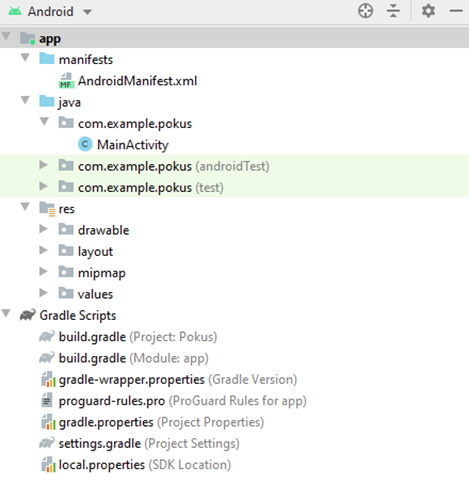
\includegraphics[scale=0.5]{images/5.jpg}
\caption{Adresářová struktura Android Studio}
\label{5}
\end{figure}
\newpage
\subsubsection{Uživatelské rozhraní}
Na obrázku níže je znázorněna struktura hlavního okna Android Studia. Je důležité znát vývojové prostředí, ve kterém zrovna programuje. I když se to nezdá, tak se jednotlivá vývojová prostředí od sebe liší, i když se jedná převážně o grafický desing IDE.
 \begin{figure}[h!]
\centering
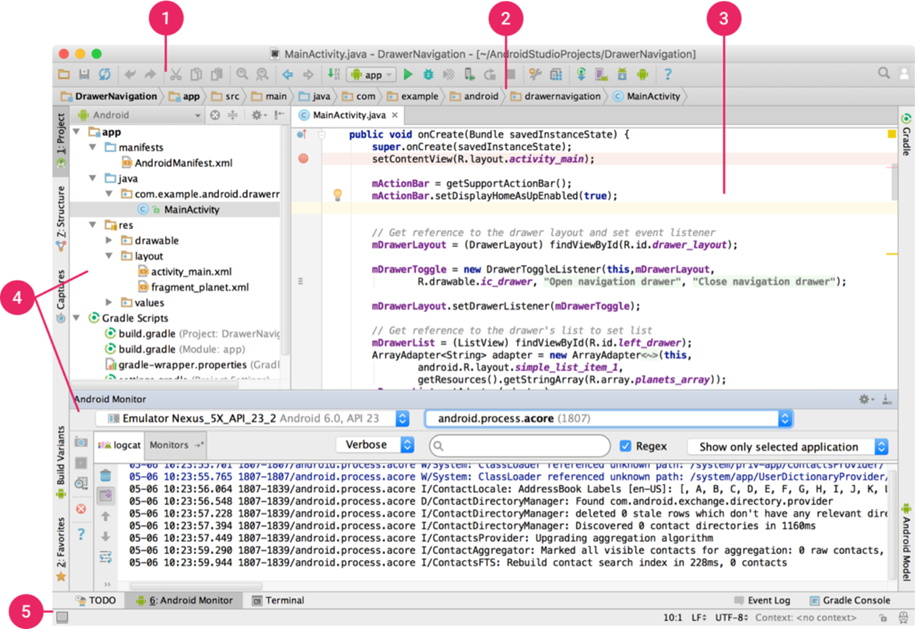
\includegraphics[scale=0.5]{images/6.jpg}
\caption{Uživatelské rozhraní Android Studio IDE}
\label{6}
\end{figure}


\begin{enumerate}
\item \textbf{Toolbar}umožňuje provádět širokou škálu akcí, jako spouštění a pozastavení projektu vytvoření AVD, debugging apod.\cite{1},\cite{17} 

\item \textbf{Navigation Bar} umožňuje pohodlně procházet projekt, otevírat, zavírat a upravovat soubory. Umožnuje tak vývojářům pohodlnější zobrazení adresářové struktury z Tool Window.\cite{1},\cite{17} 
\item \textbf{Editor Window}slouží k zobrazení aktuálního souboru, ve kterém je psán zdrojový kód. \cite{1},\cite{17} 
\item \textbf{Tool Window} umožnuje přístup k potřebným úkolům mezi které patří správa projektu, vyhledávání nebo správa verzí.\cite{1},\cite{17}  
\item \textbf{Status Bar} slouží k zobrazování aktuálního stavu IDE, zpráv nebo upozornění o aktuálním stavu aplikace. Pokud vyjde nová verze IDE nebo se nepodaří projekt správně zkompilovat, objeví se varování právě zde.\cite{1},\cite{17} 
\end{enumerate}

\subsection{Java Development Kit (JDK)}
Java Development Kit (JDK) je soubor základních nástrojů a knihoven pro vývoj aplikací a apletů pro platformu Java a Kotlin. Základní součástí JDK je Java Runtime Environment (JRE), jež slouží pro spouštění aplikací i vývojových nástrojů dále překladač, debugger atd. Jelikož se aplikace pro Android programují primárně v jazycích Java a Kotlin, je potřeba JDK, resp. JRE nainstalovat.\cite{1},\cite{11},\cite{17},\cite{18}  

 \begin{figure}[h!]
\centering
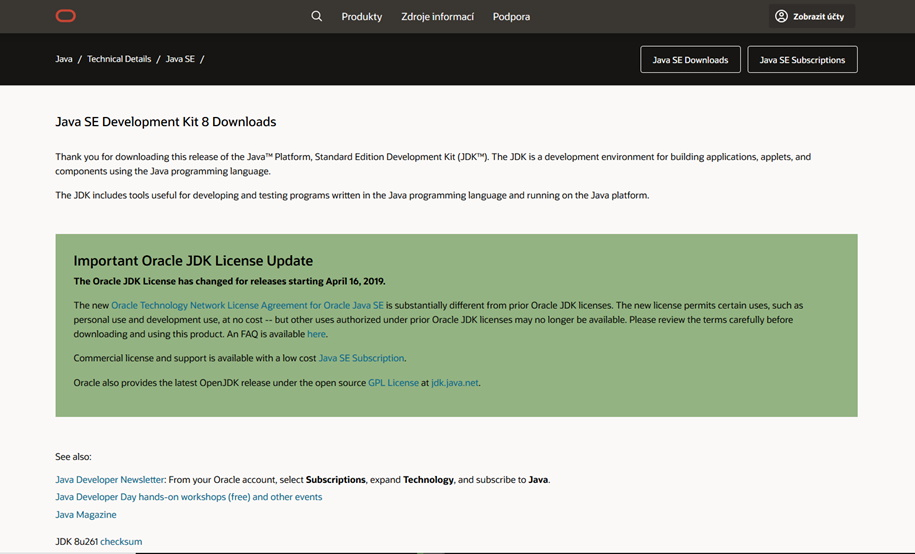
\includegraphics[scale=0.5]{images/7.jpg}
\caption{Webová stránka Java SE Development Kit 8 (JDK)}
\label{7}
\end{figure}
\newpage
\subsection{Android SDK}
Jedná se o sadu nástrojů, která zahrnuje všechny potřebné nástroje pro vývoj aplikací a její debugování. Dříve, když programátor vyvíjel aplikace v Eclipse IDE, musel si balíček SDK stáhnou zvlášť. To se ovšem změnilo příchodem Android Studia, které se už naistaluje automaticky při instalaci IDE.  Pro správu SDK se používá SDK Manager, který je součástí vývojového prostředí.

 \begin{figure}[h!]
\centering
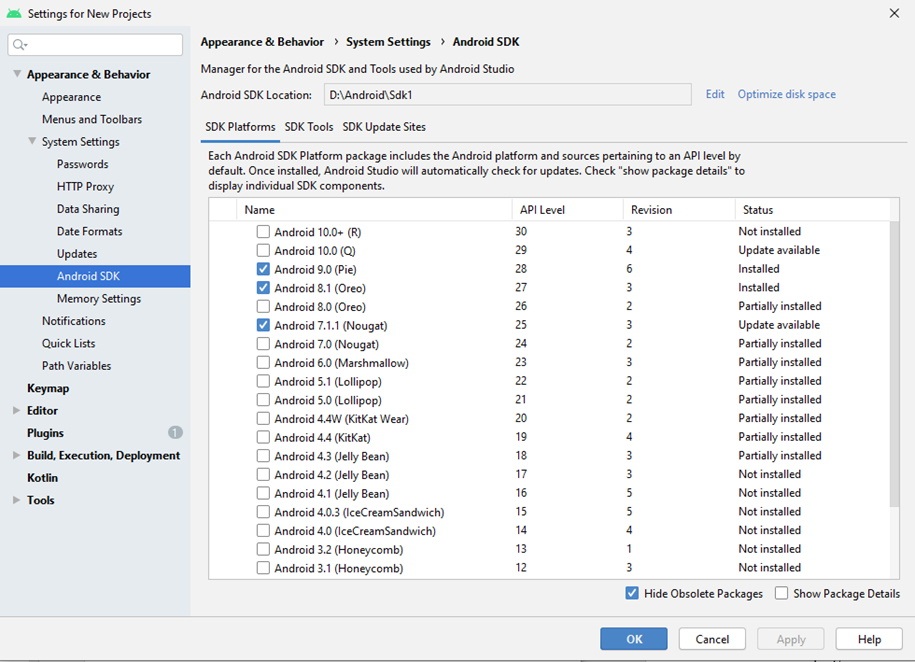
\includegraphics[scale=0.5]{images/8.jpg}
\caption{SDK Manager v Android Studio IDE}
\label{8}
\end{figure}
\newpage
\subsection{Java}
Java je objektově orientovaný programovací jazyk (OOP), který vyvinula firma Sun Microsystems v 90. letech minulého století. Jedná se v současné době o jeden z nejpopulárnějších a nejvyužívanějších programovacích jazyků. Díky své unikátní konstrukci mohou programátoři své programy spouštět na stolním počítači, webových serverech nebo na mobilních telefonech (Android). Java kód je možné částečně kompilovat a částečně interpretovat. Javovský zdrojový kód se nepřekládá do strojového kódu, jako je tomu např. u jazyku C++, ale překládá se do byte codu. „Bajtkod“ se pak překládá pomocí speciálního programu, který se nazývá Java Virtual Machine, zkráceně JVM. Díky tomuto virtuálnímu stroji lze program spustit na různých operačních systémech – MS Windows, Linux OS nebo macOS.\cite{5},\cite{7},\cite{13},\cite{14},\cite{15},\cite{16}    

 \begin{figure}[h!]
\centering
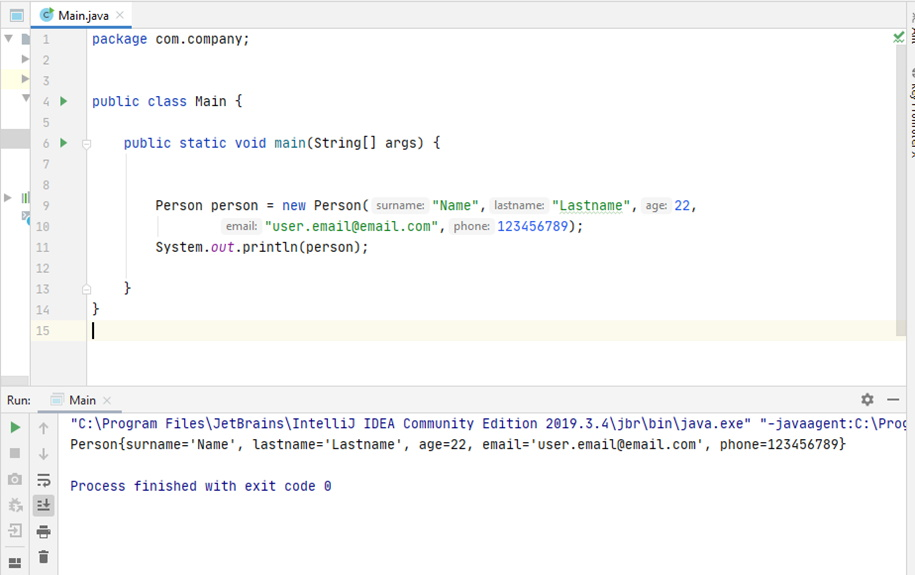
\includegraphics[scale=0.5]{images/9.jpg}
\caption{Main.java v jazyku Java}
\label{9}
\end{figure}

 \begin{figure}[h!]
\centering
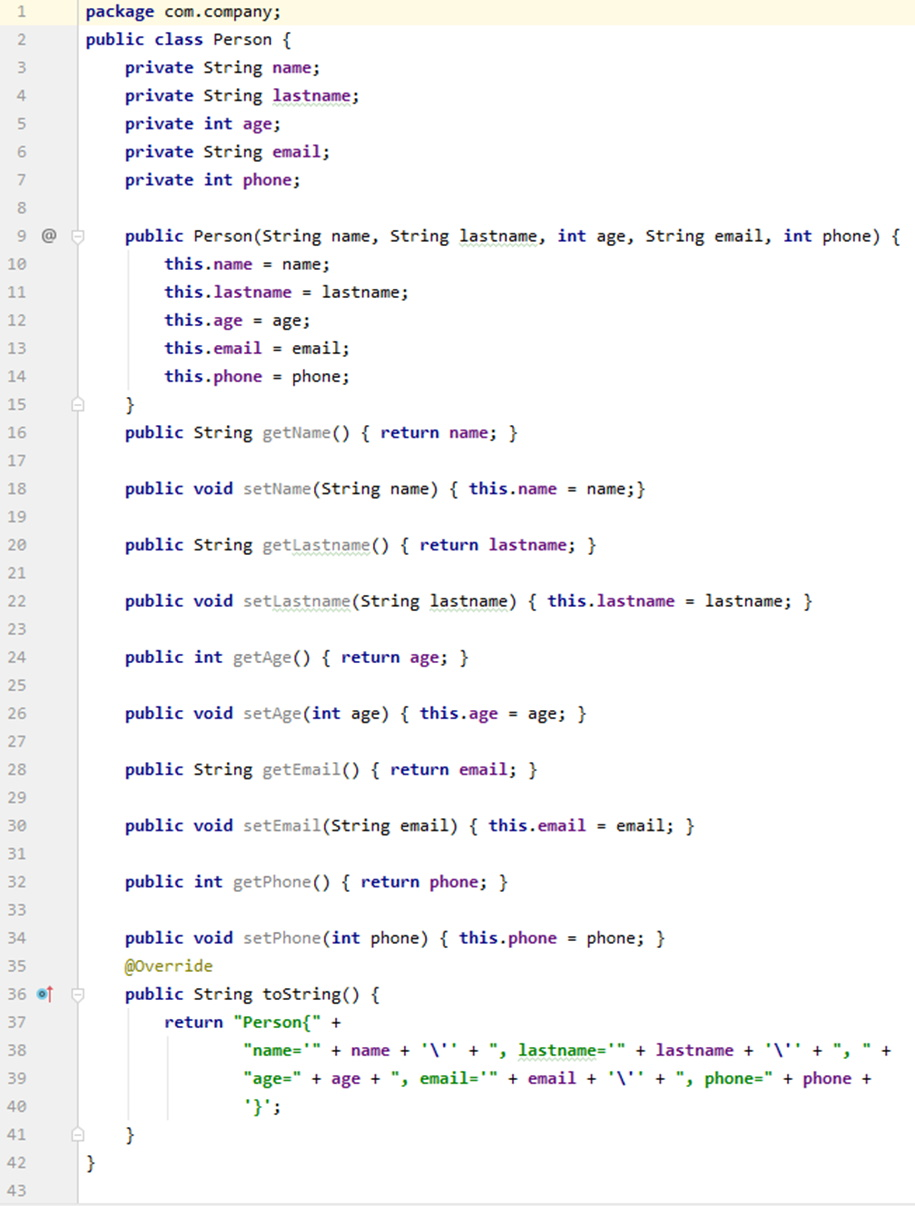
\includegraphics[scale=0.5]{images/10.jpg}
\caption{Ukázka Person.java v jazyku Java}
\label{10}
\end{figure}

\newpage
\subsection{Kotlin}
Kotlin je nový programovací jazyk vytvořený formou JetBrains, která stojí za vytvořením IntelliJ IDEA a Android Studio. Jedná se o staticky typovaný programovací jazyk, který je primárně zaměřený na Java Virtual Machine a JavaScript. V mnoha literaturách se lze dočíst, že se jedná hlavně o funkcionální jazyk, v podstatě je ale Kotlin objektově orientovaný jazyk (OOP), který podporuje funkcionální programování. Mezi hlavní výhody Kotlinu patří bezpečnost, jednoduchost a velká podobnost s jazyky Java a C\#. Ovšem mezi hlavní výhody patří vynechání středníku na konci příkazu, což hodně programátorů uvítalo. Při překladu zdrojového kódu totiž patří mezi nejčastější důvod chybného zkompilování právě středník, který jsme zapomněli vložit.\cite{6} 

 \begin{figure}[h!]
\centering
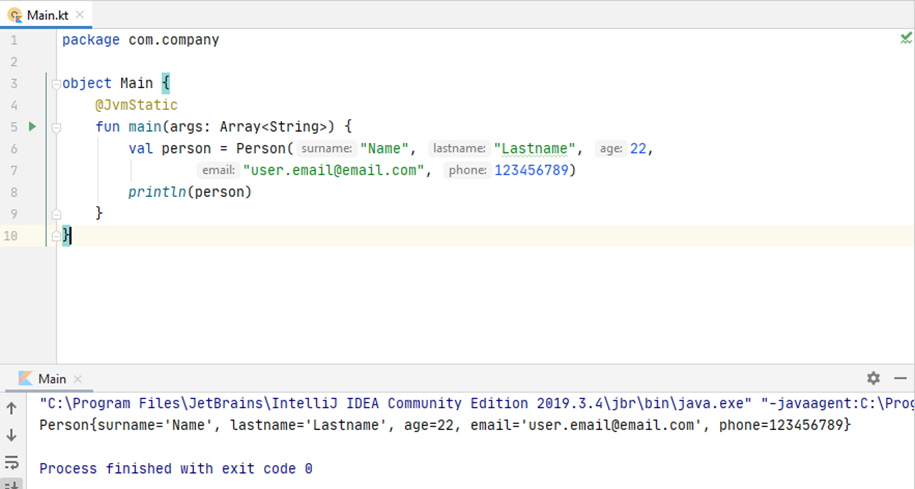
\includegraphics[scale=0.5]{images/11.jpg}
\caption{Main.kt v jazyku Kotlin}
\label{11}
\end{figure}

 \begin{figure}[h!]
\centering
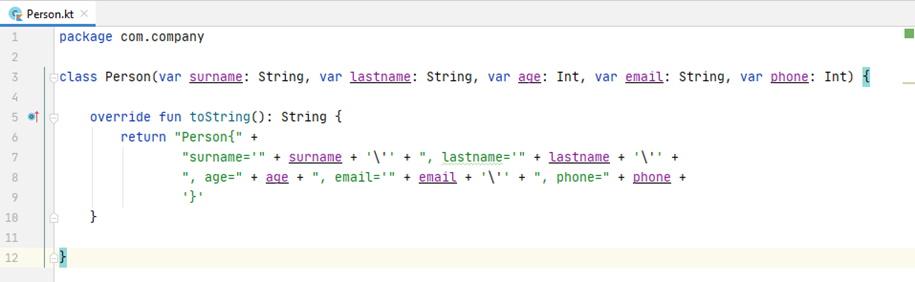
\includegraphics[scale=0.5]{images/12.jpg}
\caption{Ukázka Person.kt v jazyku Kotlin}
\label{12}
\end{figure}

\subsection{XML}
Jazyk XML (eXtensible Markup Language) je rozšiřitelný značkovací jazyk, který byl vyvinut a standardizován konsorciem W3C. Jedná se o zjednodušenou podobu staršího jazyka SGML. Umožňuje snadné vytváření konkrétních značkovacích jazyků (tzv. aplikací) pro různé účely různých typů dat. K hlavní výhodě jazyka patří multiplatformovost a univerzálnost.\cite{8} 

 \begin{figure}[h!]
\centering
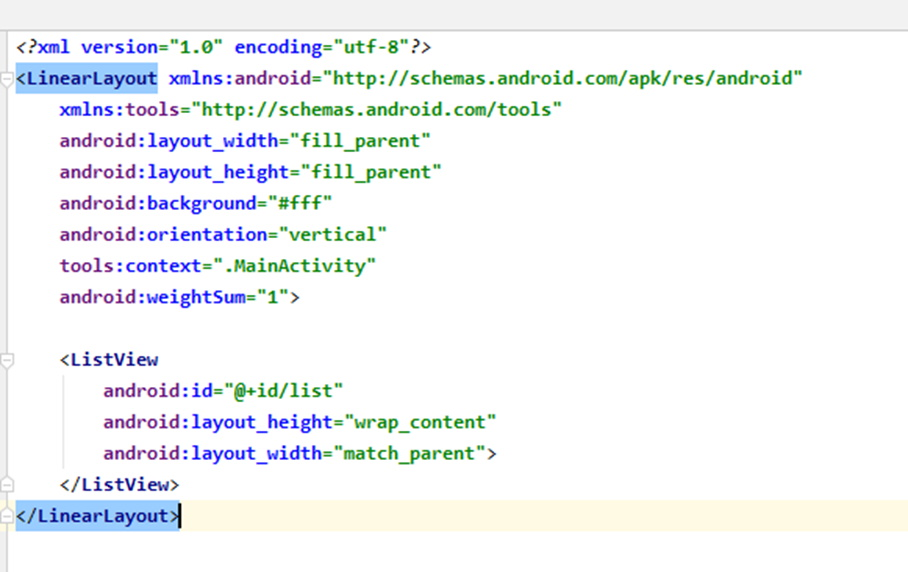
\includegraphics[scale=0.5]{images/13.jpg}
\caption{Ukázka XML}
\label{13}
\end{figure}
\newpage
\subsection{SQLite}
SQLite reprezentuje relační databázový systém, jenž je obsažen v jedné malé knihovně. Jedná se o systém, který je velmi šetrný k paměti zařízení a poměrně rychlý, což je velká výhoda při použití v zařízeních jako jsou např. mobilní telefony. Další výhodou této relační databáze je její snadná použitelnost v rámci aplikace, jelikož SQLite nepracuje na principu klient-server, jako jiné databázové systémy.\cite{9} 
 
 \begin{figure}[h!]
\centering
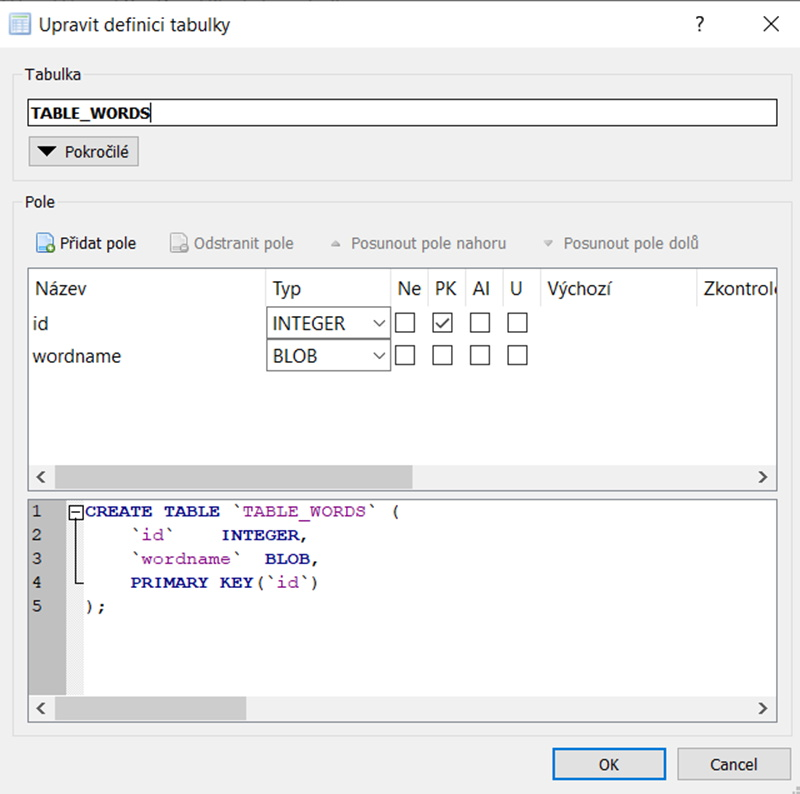
\includegraphics[scale=0.4]{images/14.jpg}
\caption{Ukázka SQLite v DB Browseru}
\label{14}
\end{figure}

%\input kapitola2.tex

%\csname JS@pagefig\endcsname{page16}{vskpou-src.pdf}\advance\count0 1

%\subsection{Podkapitola}
%A zde se odkazuji na \cite{Knuth}.







%%%%%%%%%%%%%%%%%%%%%%%%%%%%%%%%%%%%%%%%%%%%%%%%%%%%%%%%%%%%%%%%%%%%%%%%%
\section{NÁVRH APLIKACE}
Tato část práce je věnovaná samotnému návrhu aplikace.
%\input kapitola3.tex
\subsection{Základní informace}
Všichni vývojáři, než se pustí do vývoje, si musí nejprve určit priority, jako programovací jazyk a vývojové prostředí.  Toto rozhodnutí je nesmírně důležité, protože může ovlivnit samotný vývoj. V mém případě jsem zvolil pro vývoj Android Studio. Za programovací jazyky jsem si zvolil Javu, Kotlin a XML. 

\subsection{Existující aplikace }
V Google Play existuje celá řada aplikací, které slouží jako manuál pro tvorbu aplikací. Nechci tím říct, že jsou špatné, ale všechny mají jeden společný problém. A tím problémem je, že jsou v angličtině. Toto beru jako velký nedostatek, a proto jsem se rozhodl to napravit. Ať už se jedná o vývoj mobilních aplikací nebo webových aplikací, je dobré se vždy podívat na již exitující aplikace. Získáte tak informace o tom, co dělá aplikaci dobrou (tyto prvky pak použijete ve své aplikaci), a nebo špatnou (tyto prvky do aplikace nepoužijete nebo se je pokusíte opravit).

\subsubsection{Learn Android Tutorial – Android App Development}
Learn Android Tutorial považuji asi za jednu z nejlepších „tutorial“ aplikací. Velkou výhodou této aplikace je, že je zcela zdarma, a navíc oproti jiným aplikacím může běžet zcela v offline režimu, takže nepotřebuje připojení k internetu. Při tvorbě své aplikace mi Learn Android Tutorial posloužil jako vzor, co se týká zobrazování menu nabídky. V rámci vývoje jsem se snažil aplikovat nedostatky jak této, tak stávajících aplikace. Mezi hlavní nevýhody této aplikace považuji:

\begin{enumerate}
\item {Vysvětluje vývoj aplikací pouze v Javě.}

\item {Celá aplikace popisuje vývoj v anglickém jazyce.} 

\end{enumerate}
\\
Celá aplikace Learn Android Tutorial – Andrpif App Development je rozdělena na:
\\
\begin{itemize}
    \item {Tutorial} -- potřebná teorie o Androidu,
    \item {Basic Examples} -- jednoduché ukázky příkladů jako je: Menu; UI Widgets, Intents, atd,
    \item {Advance Example} -- praktické příklady,
    \item {Interview Q/A} -- nejčastější otázky na Android, příkazy a jejich stručné odpovědi,
    \item {Quiz} -- prověření uživatelových znalostí,
    \item {Tips and Tricks} -- tipy a triky pro vývoj,
    \item {Share} -- možnost sdílení aplikace.
\end{itemize}

 \begin{figure}[h!]
\centering
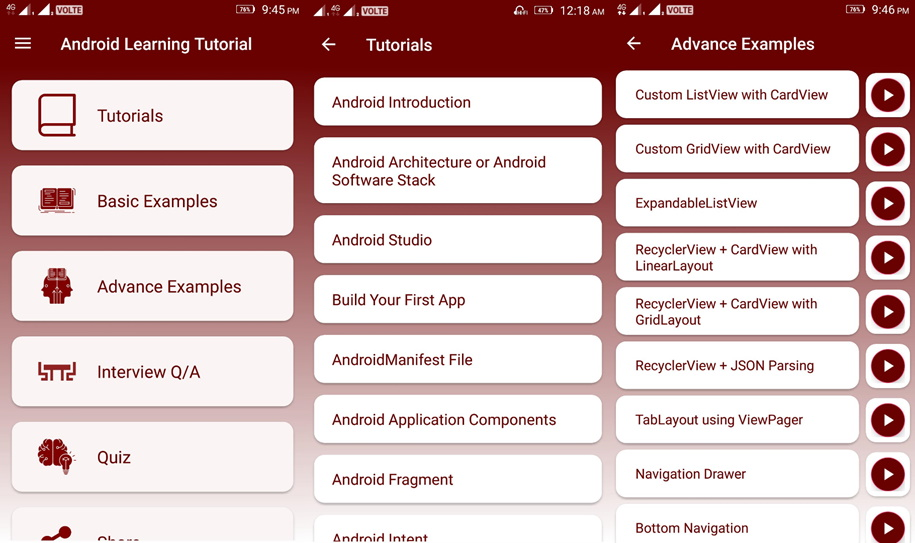
\includegraphics[scale=0.4]{images/15.jpg}
\caption{Learn Android Tutorial – Android App Development}
\label{15}
\end{figure}

\subsection{Návrh aplikace}
Zadání aplikace patří mezi nejdůležitější část celého návrhu každé aplikace. Pokud se přesně nenadefinují požadavky aplikace, může toto chybné zadání vést k fiasku aplikace. Pokud vytvoříme něco, s čím klient nesouhlasí, nemusí nám za náš výtvor zaplatit. Proto je důležité si přesně nadefinovat požadavky, které má aplikace splňovat. Celý návrh se dělí do dvou skupin: funkční a nefunkční požadavky. Mezi funkční požadavky patří dané body, které musí aplikace mít (to, co si klient přesně přeje). Mezi nefunkční požadavky patří např. OS, na kterém se bude aplikace vyvíjet, programovací jazyk atd.



\begin{table}[h]
\begin{center}
\begin{tabular}{ |c|c| }



\hline
{\centering}\textbf{Funkční požadavky}&
{\centering}\textbf{Nefunkční požadavky}
 \\
\hline
Vzdělávací aplikace&
Windows 10
 \\
\hline
Android OS&
Java, Kotlin
 \\
\hline
Manuál&
Notebook \\
\hline
Programování&
 \\
\hline
Android - Java a Kotlin&
 \\
\hline
čeština&
 \\
\hline


\end{tabular}
\caption{Funkční a nefunkční požadavky}
\end{center}
\end{table}


Z tabulky vyplývá, že zadání mé aplikace zní: Vytvořit vzdělávací mobilní aplikaci pro Android OS, která bude sloužit jako manuál pro vývoj mobilních aplikací pro Android OS v jazycích Java a Kotlin a celý manuál bude v češtině.
\newpage
\subsection{Volba jazyka}
Než jsem se pustil do tvorby aplikace, měl jsem před sebou velký problém. Jaký programovací jazyk zvolit. Jak jsem se již zmínil, pro tvorbu nativní aplikace se používají dva programovací jazyky, Java a Kotlin. Java patří mezi nejpoužívanější programovací jazyky a díky své konstrukci se řadí mezi multiplatformní jazyk. Díky této výhodě si ho Google vybral jako primární a zároveň oficiální programovací jazyk pro tvorbu mobilních aplikací. To se však změnilo v roce 2017 na změnilo, kdy po 10 letech Javu nahradil Kotlin.

 \begin{figure}[h!]
\centering
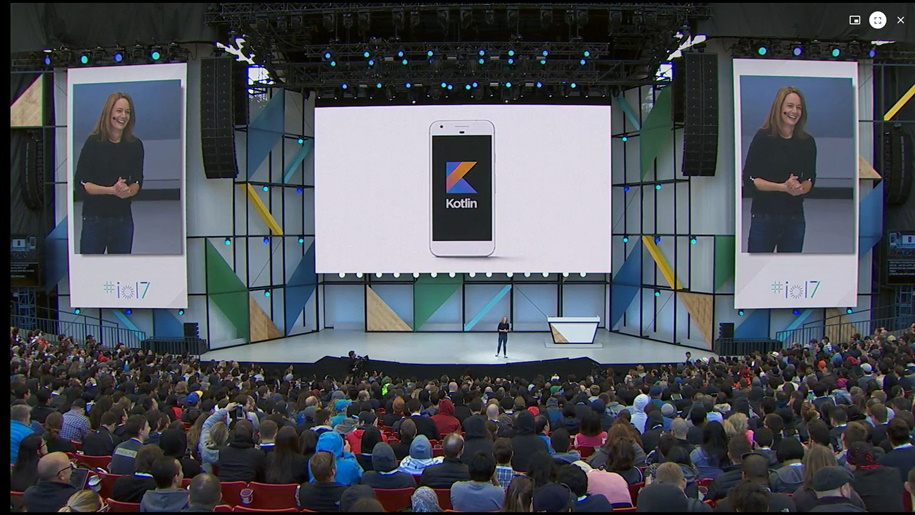
\includegraphics[scale=0.5]{images/16.jpg}
\caption{Onzámení Kotlinu jako primární jazyk na Google I/O 17}
\label{16}
\end{figure}
\\
Tím došlo k rozdělení Android vývojářů na dva tábory:\\

\begin{enumerate}
\item {Java vývojáře}

\item {Kotlin vývojáře} 

\end{enumerate}
\\
Tak který si vybrat? Osobně doporučuji používat oba dva. Více než 80 \% Android aplikací jsou naprogramovány v Javě, a proto se firmám vyplácí udržovat a spravovat aplikace v Javě, než je přeprogramovat do Kotlinu. Ovšem když se chcete pustit do nové aplikace, doporučuje se ji psát v Kotlinu. Ovšem je tu i další možnost, a to je psát aplikace v obou jazycích. Kotlin totiž vychází z Javy, a proto je možné během vývoje používat hotové javovské knihovny. Navíc, pokud narazíte na určitý problém, který nedokážete vyřešit v Kotlinu nebo ho dokonce Kotlin neumí řešit, můžete část aplikace napsat v Javě.\\\\ Proto jsem se rozhodl vytvořit svou aplikace v Javě a zároveň v Kotlinu, abych tak ukázal využití těchto jazyků při tvorbě aplikace.\\

\newpage
\subsection{Příprava a vytvoření nového projektu}
Než se pustíme do samotné tvorby aplikace, je nutné si stáhnout potřebné IDE. Pro tvorbu aplikací jsem stejně jako každý současný android programátor zvolil Android Studio. Stačí je pouze stáhnout ze stránky \url{https://developer.android.com/studio/index.html} a nainstalovat ho. Oproti vývoji mobilních aplikací pro iOS, kde je zapotřebí vlastnit Apple zařízení s Mac OS, má vývoj pro Android značně velkou výhodu. Umožňuje vyvíjet aplikací na všech dostupných platformách (Microsoft Windows, Linux OS a Mac OS). Po stáhnutí a otevření instalačního balíčku se program jednoduše naistaluje Pokud si nevíte rady s instalací nebo během ní došlo k problému, máte možnost vyhledat pomoc na internetové stránce \url{https://developer.android.com/studio/install.html}, kde máte i podrobný manuál, jak postupovat při instalaci na různých platformách.\\
\\
Po úspěšném nainstalování se Android Studio otevře. Popis, čím vším je nutné se proklikat zde neuvádím. Je to poměrně pracná činnost a věřím, že po prostudování manuálu, na který jsem již vložil odkaz to každý zvládne. Během instalace se nabízí možnost vytvořit i AVD (Android Virtual Devices), které simuluje reálné mobilní zařízení. Tuto možnost vytvoření mohu jenom doporučit. Při testování aplikace není nutné svůj projekt exportovat a nahrát do fyzického zařízení, ale je možné si projekt jednoduše spustit AVD.\\
\\
Po úspěšném dokončení potřebného nastavení se zobrazí nabídka s možností vytvoření nového projektu. Jakmile tak učiníme, zobrazí se nám další důležité okno, Configure Your Project, viz obrázek č.~\ref{17}.

 \begin{figure}[h!]
\centering
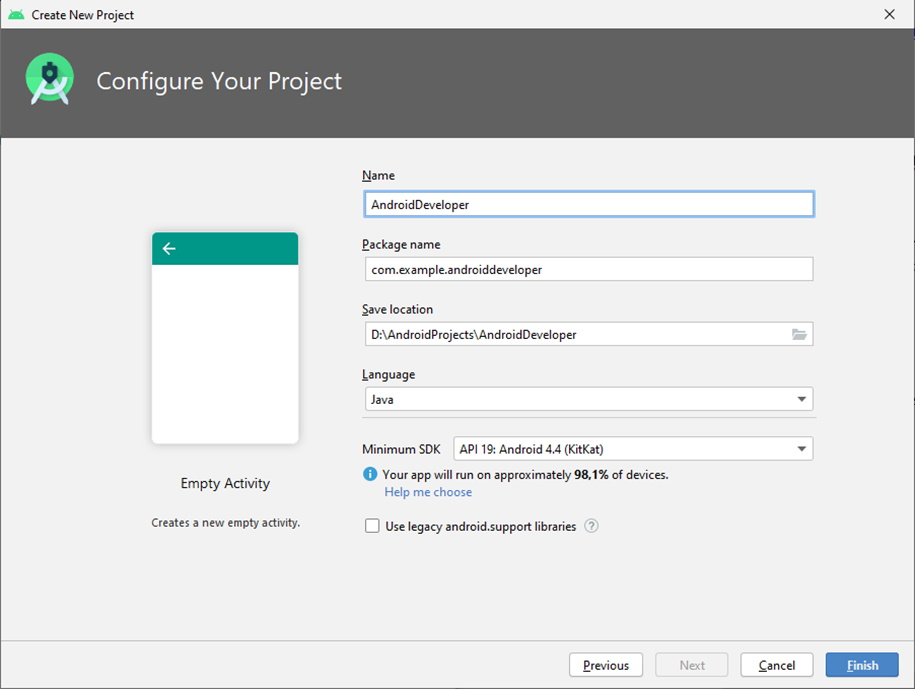
\includegraphics[scale=0.5]{images/17.jpg}
\caption{Vytvoření nového projektu v Android Studiu}
\label{17}
\end{figure}
\newpage
V tomto kroku patří mezi nejdůležitější body:

\begin{itemize}
    \item {Name},
    \item {Save location},
    \item {Language},
    \item {Minimum SDK}. 
   
\end{itemize}
\\
U názvu je velmi důležité, aby byl název unikátní (jedinečný). Kdybychom tak neučinili, výsledek by měl katastrofální následky. Při vytvoření několika projektů se stejným názvem by došlo ke sloučení projektů a jen těžko bychom se vyznali. Já jsem si aplikaci pojmenoval Android Developer.\\
\\Dalším krokem je pak umístění projektu. Projekt si je možné uložit kamkoliv, ovšem Android Studio stejně jako IntelliJ IDEA nebo Eclipse nabízí možnost ukládat soubory do složky, kterou vývojové prostředí samo vytvoří pro tyto účely. V mém případě se jedná o složku AndroidProject.\\
\\V dalším kroku je třeba zvolit programovací jazyk. Pro Android si můžeme vybrat ze dvou primárních jazyků, a to Javy a Kotlinu. Pokud vyvíjíte aplikace sami, je volba jazyka na Vás, ale pokud pracujete v týmu, musíte pracovat v jazyku, na které se předem domluvíte. Já pro svou aplikaci používám oba jazyky, nicméně pro vytvoření projektu jsem vybral Javu.\\
\\V posledním kroku je definováno minimální SDK (minimum SDK). Pokud je zvolena nižší verze SDK, je větší šance, že aplikace poběží na většině zařízení. Pro svou aplikaci jsem nastavil minimální SDK na API 19 (Android 4.4 – KitKat).

 \begin{figure}[h!]
\centering
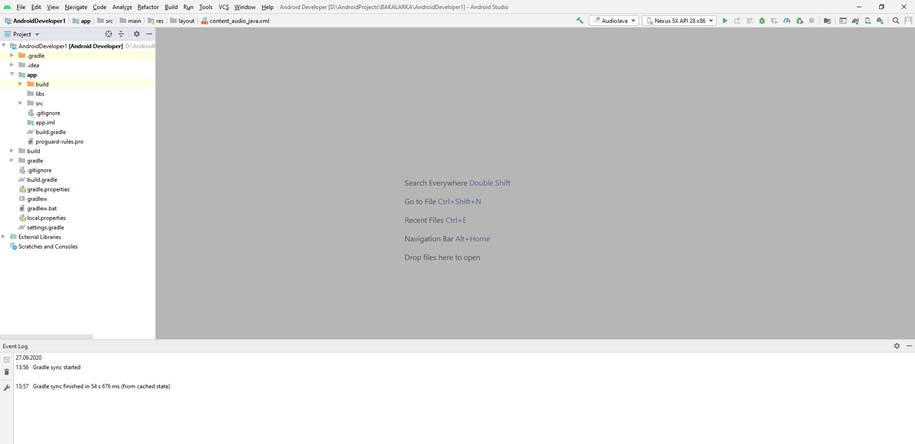
\includegraphics[scale=0.5]{images/18.jpg}
\caption{Ukázka připraveného IDE pro vývoj}
\label{18}
\end{figure}

Po vytvořen nového projektu se zobrazí toto okno. Jedná se hlavní okno celého Android Studio IDE. Pokud se toto okno zobrazí, úspěšně se tak podařilo dokončit instalaci a můžeme se pustit do vývoje.



\subsection{Tvorba aplikace}
Jak jsem se již dříve zmínil v části 3.3 Návrh demonstrativní aplikace, mám za úkol naprogramovat aplikaci v českém jazyce, která poslouží jako manuál pro vývoj mobilních aplikací pro Android.\\
\\
Dalším krokem je úkol, jak zobrazit všechny příklady např. kalkulačku, video přehrávač, galerii v jedné aplikaci? V odborné literatuře nebo ve video tutoriálech tvoří každý takový příklad svou vlastní aplikaci. I na to má Android svůj způsob řešení. Na rozdíl od desktopové aplikace, kde by se to muselo složitě zabudovávat do kódu, Android umožňuje propojit několik aplikací do jedné \textbf{VELKÉ} aplikace. Jelikož se můj návrh aplikace skládá z několika menších aplikací, rozhodl jsem se popsat prvky, které jsme použil při tvorbě hlavní části aplikace, tj. zobrazovací menu celé aplikace (viz. obrázek níže), protože jednotlivé příklady včetně zdrojových kódů jsou popsány v samotné aplikaci.

 \begin{figure}[h!]
\centering
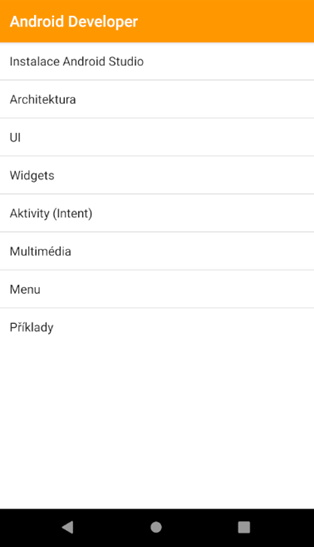
\includegraphics[scale=0.5]{images/19.jpg}
\caption{Ukázka ListView v ukázkové aplikaci}
\label{19}
\end{figure}
\\
\\Kromě programovacích jazyků Java a Kotlin bylo nutné použít několik rozšiřujících doplňků potřebných pro funkčnost, ovladatelnost a správný chod aplikace. Než jsem se pustil do samotného vývoje, určil jsem potřebné priority, které chci, aby tak aplikace fungovala podle mých představ. Jak by aplikace měla fungovat? Po kliknutí aplikace se uživateli zobrazí seznam jednotlivých tutoriálů. Po výběru daného tutoriálu se uživateli zobrazí demonstrující příklad a po kliknutí ikony pro zobrazení zdrojového kódu se zobrazí zdrojový kód daného příkladu v jazycích Java, Kotlin a XML. Takto by aplikace měla fungovat. Pro realizaci tohoto chodu jsem použil Activity, ListView a Intent. Důvod, proč jsem použil tyto komponenty jsou popsány níže.
\\
\newpage
\textbf{Android prvky}
\begin{itemize}
    \item \textbf{ListView}\\
    Android ListView je kontejner, který slouží k zobrazení několika položek v rolovacím seznamu. Typickým příkladem, kde se můžeme uživatel setkat se zobrazením ListView je seznam SMS zpráv nebo seznam kontaktů v mobilu. Pro zajištění zobrazení položek, používá Android tzv. Adapter. Tento Adapter zajistí propojení jednotlivých položek seznamu ve správném pořadí tak, jak jsem si ho sám nadefinoval. Pro seznam je dobré použít patřičnou datovou strukturu, v mém případě pole datového typu string. Důvodem, proč jsem použil datovou strukturu pole je v tom, že se mi zobrazí položky v seznamu přesně tak jak chci, tj. na první pozici se mi zobrazí Instalace Android Studio, na druhé pozici Architektura, atd. Jedná se tak o pevné umístění položek, které uživatel nemůže v aplikaci změnit (např. změnit jejich pořadí). To může pouze programátor ve zdrojovém kódu.
        \begin{figure}[h!]
        \centering
        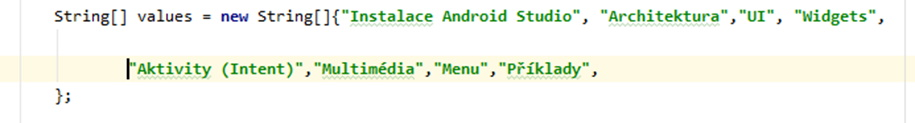
\includegraphics[scale=0.5]{images/20.jpg}
        \caption{Datová struktura s položkami, které se mají zobrazit v ListView}
        \label{20}
        \end{figure}
        \\
        Když je nadefinovaná datová struktura, přichází na řadu její propojení s Adaptérem. Kromě nadefinování datového typu, jména a vytvoření nového objektu musí Adaptér obsahovat čtyři parametry. Jedná se o Context (kontext), resource (zdroj) a object (objekt).\\
        
        
        
            \begin{table}[h]
            \begin{center}
            \begin{tabular}{ |p{3cm}|p{3cm}|p{6cm}| }
            
            
            
            \hline
            {\centering}\textbf{Parametr:}&
             {\centering}\textbf{Význam:}&
             {\centering}\textbf{Příkaz ve zdrojovém kódu}
             \\
            \hline
           Context&
            Slouží jako odkaz na aktuální třídu, ze které se budou data získávat.&
            this
             \\
            \hline
           resource&
            ID prostředku pro potřebné rozložení.&
            %\verb|simple_list_item1|
            android.R.layout.simple\_list\_item1
            
             \\
            \hline
            object&
            Jedná se o objekt, jehož data se mají zobrazit.&
            listOfItems\\
            \hline
           
            \end{tabular}
            \caption{Tabulka požadavků pro aplikaci}
            \end{center}
            \end{table}
        
        
        
        
        
        

        \begin{figure}[h!]
        \centering
        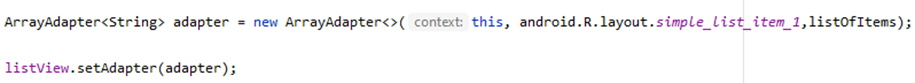
\includegraphics[scale=0.5]{images/21.jpg}
        \caption{Propojení datové struktury s adapterem}
        \label{21}
        \end{figure}
        \\
        Pomocí příkazu listView.setAdapter(adapter) pak už stačí propojit Apadpter s XML souborem, který je naprogramovaný jako rolovací seznam (viz obrázek).\\
        \\
                \begin{figure}[h!]
        \centering
        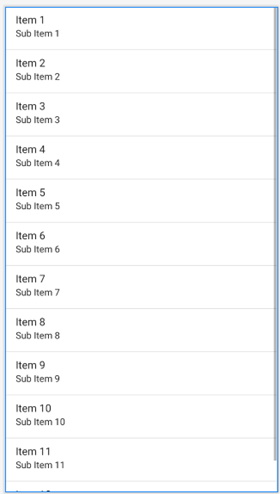
\includegraphics[scale=0.5]{images/22.jpg}
        \caption{Ukázka ListView pomocí XML v Android Studiu}
        \label{22}
        \end{figure}\\
        
        \begin{figure}[h!]
        \centering
        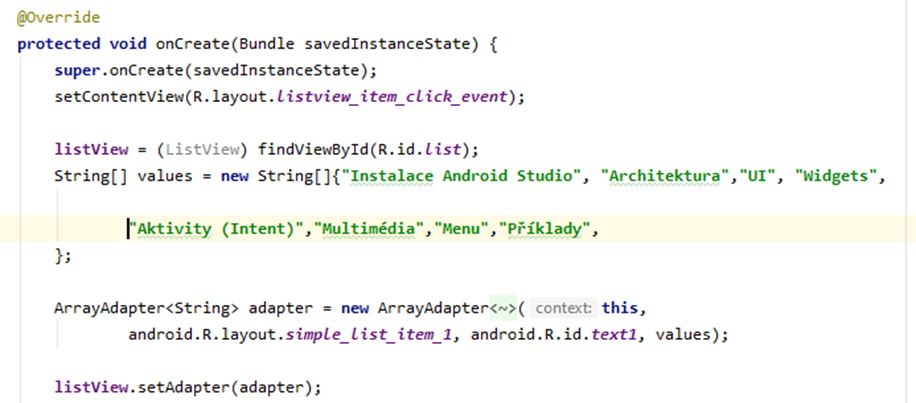
\includegraphics[scale=0.5]{images/23.jpg}
        \caption{Ukázka třídy ListItem.java v jazyku Java z aplikace}
        \label{23}
        \end{figure}\\
        
        \begin{figure}[h!]
        \centering
        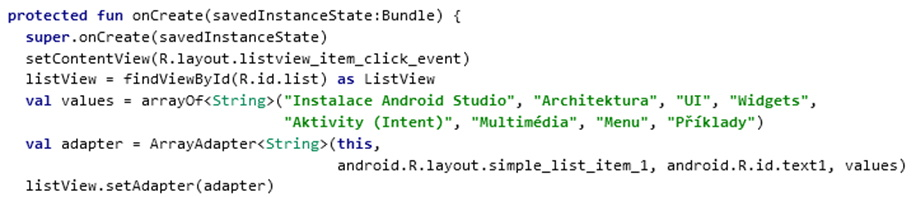
\includegraphics[scale=0.5]{images/24.jpg}
        \caption{Ukázka třídy ListItem.ktv jazyku Kotlin z aplikace}
        \label{24}
        \end{figure}
    \newpage   
    \clearpage  
    \item \textbf{Aktivity}
    \\
    V Android světě slouží Aktivity jako hlavní třída, která se po spuštění aplikace spustí hned jako první. Můžeme říct, že se jedná o jeden ze stavebních kamenů všech Android aplikací. Aktivity umožňují pohodlnou komunikaci mezi uživatelem a samotnou aplikací. Všechny aplikace se zpravidla skládají z více aktivit, které jsou mezi sebou navzájem propojeny\\
    \\Ať už programujeme v jazyku C, C++, C\#, Java nebo Kotlin, pro spuštění programu používáme metodu main(). Stejným způsobem spouštíme aplikace i v Android, s tím rozdílem, že se metoda jmenuje onCreate(). Není to ovšem jediná metoda Aktivity, je jich celkem 7.\\
    \textbf{Metody Aktiviry:}
    
        \begin{itemize}
        \item \textbf{onCreate():} -- metoda, která se volá hned po vytvoření aktivity;
        \item \textbf{onStart():} -- metoda, která se volá, když se uživatel vrátí do aktivity;
        \item \textbf{onResume():} -- metoda, která se volá, když aktivita komunikuje s uživatelem;
        \item \textbf{onPause():} -- metoda, která se volá, pokud dojde k přesunutí do jiné aktivity; 
        \item \textbf{onStop():} -- metoda, která se volá v doby, kdy není aktivita viditelná pro uživatele; 
        \item \textbf{onRestart():} -- metoda, která se volá, při ukončení aktivity;
        \item \textbf{onDestroy():} -- metoda, která se volá při restartu aktivity po jejím zastavení; 
        \end{itemize}
        
        \begin{figure}[h!]
        \centering
        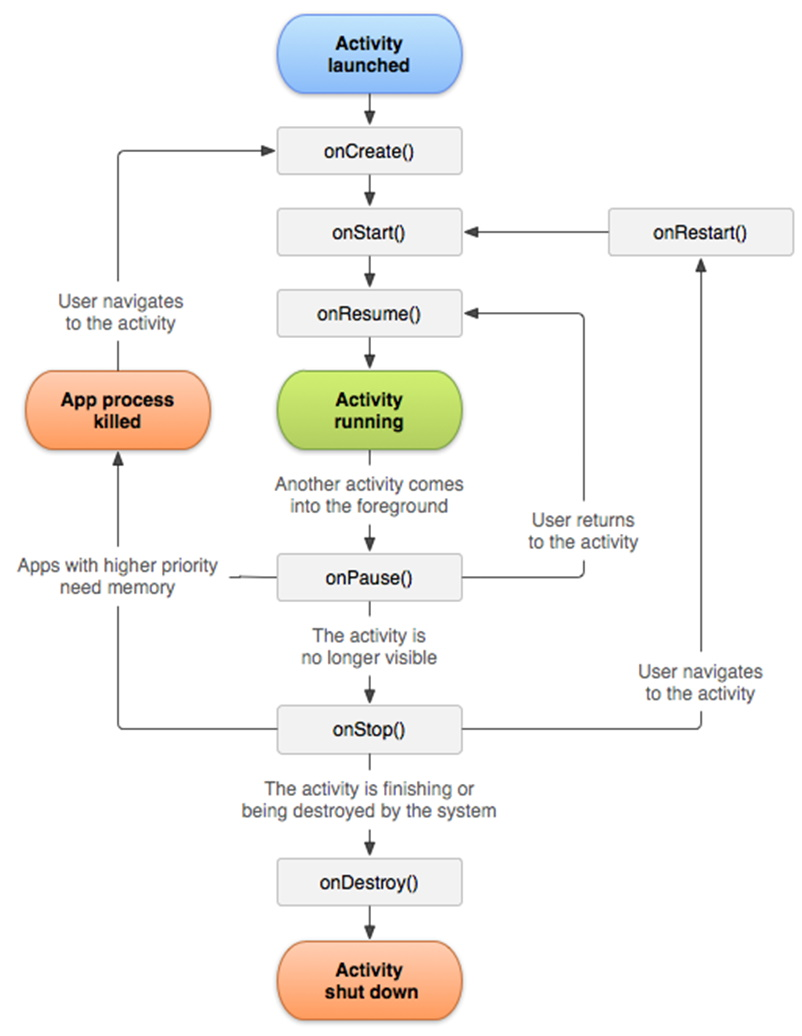
\includegraphics[scale=0.3]{images/25.jpg}
        \caption{Životní cyklus Activity}
        \label{25}
        \end{figure}
    
    \newpage
    \item \textbf{Intent}\\
    Intent je abstraktní operace, která nám slouží k vykonání určité operace. Jedná se o objekt, který v systému Android slouží pro komunikaci mezi komponentami aplikace (předávání informací mezi sebou) a přecházení z jedné aplikace do jiné aplikace. V podstatě celé aplikace se skládají z aktivity a ze zpráv mezi intenty. Intenty se převážně skládají z:
     \begin{itemize}
        \item činnost, která se má vykonat,
        \item parametr, nad kterým se má určitá činnost provést,
        \item aplikace, která má danou akci provést.
        \end{itemize}
       
     Mezi typické činnosti, které Intent provádí jsou:
    
          \begin{itemize}
        \item Vytočení a příjem hovoru -- Intent.\textit{\textbf{ACTION\_CALL}},
        \item Odesílání SMS -- Intent.\textit{\textbf{ACTION\_VIEW}},
        \item Odesílání Emailu -- Intent.\textit{\textbf{ACTION\_SEND}},
        \item Zobrazené webové stránky -- Intent.\textit{\textbf{ACTION\_VIEW}},
        \item Zahájení jiné činnost, jako např. otevření nové aktivity.
        \end{itemize}
     \newpage
          \begin{figure}[h!]
        \centering
        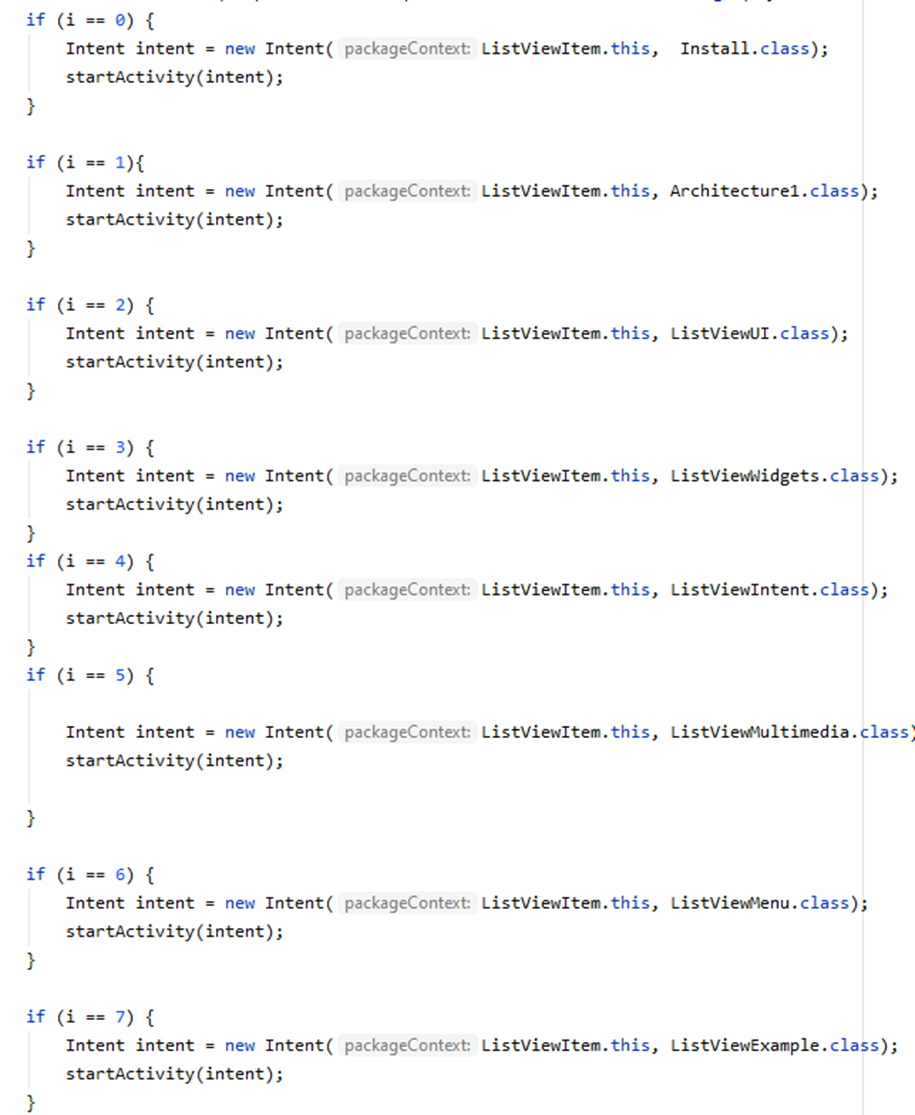
\includegraphics[scale=0.4]{images/26.jpg}
        \caption{Intent z aplikace v jazyku Java}
        \label{26}
        \end{figure}
        \newpage
        \begin{figure}[h!]
        \centering
        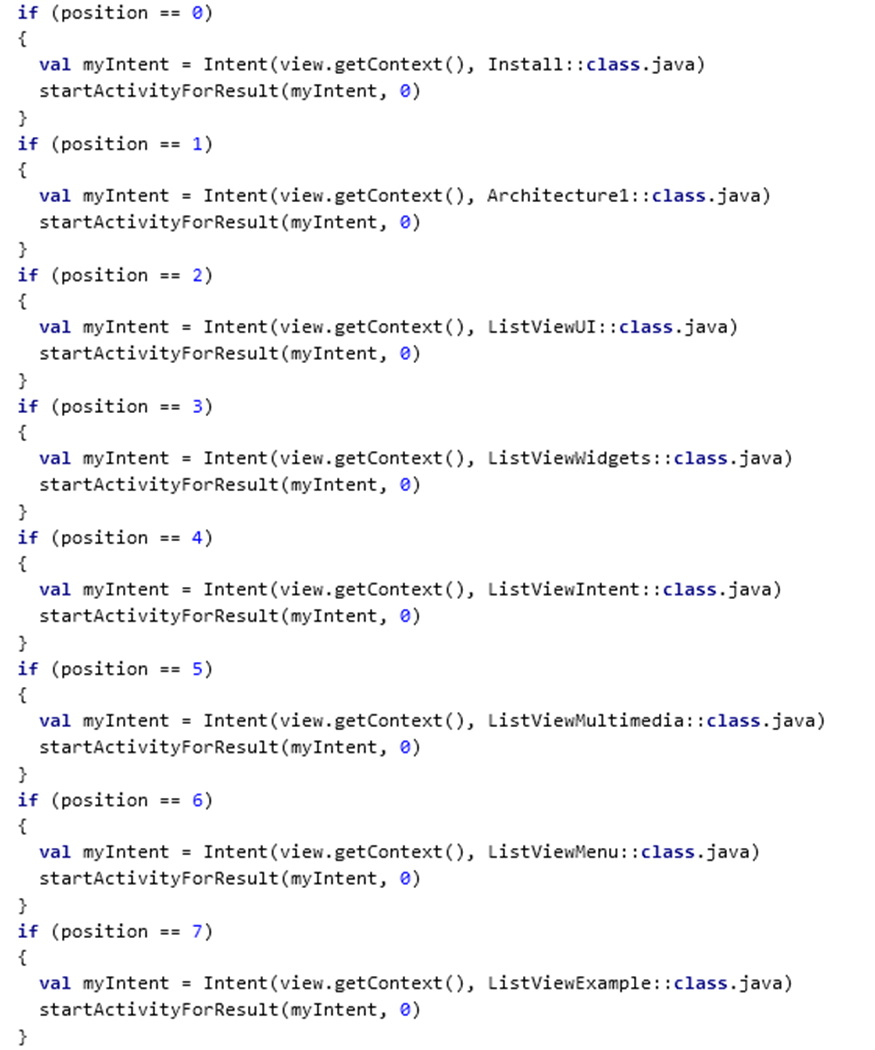
\includegraphics[scale=0.4]{images/27.jpg}
        \caption{Intent z aplikace v jazyku Kotlin}
        \label{27}
        \end{figure}
  \\
 
  Ve své aplikaci jsem použil explicitní Intent. Jedná se o Intent, který slouží k zahájení jiné činnosti, tj spuštění nové aktivity. Příkaz je velice jednoduchý. Stačí vytvořit nový objekt Intent a jako parametr (hodnoty v kulatých závorkách) je nutné uvést Context (výchozí třídu, ze které voláme) a třídu (.class), která se má spustit. Pak už stačí vyvolat tento Intent pomocí metody startActivity a do parametru vložit Intent, který se má spustit (Intent).
    \end{itemize}







\stranyresume





\addcontentsline{toc}{section}{Závěr}
\section*{Závěr}

Při tvorbě této závěrečné práce mi dělaly největší potíže tabulky a správné zobrazení obrázků tam, kde chci.


\newpage













\begin{thebibliography}{9}


%% priklad monograficke publikace:

\bibitem{1} Allen, Grant \textit{Android 4: průvodce programováním mobilních aplikací.} Brno: Computer Press, 2013. \ISBN{978-80-251-3782-6}.

\bibitem{2} Čada, Ondřej \textit{Objektové programování: naučte se pravidla objektového myšlení.} Praha: Grada, 2009. \ISBN{978-80-247-2745-5}.


\bibitem{3} Eclipse desktop \,\&\, web IDE . \textit{Eclipse desktop \,\&\, web IDE } [online].[citováno 18.\,08.\,2020].
\url{https://eclipse.org/ide/}.

\bibitem{4} GoalKicker.com. \textit{Android Notes for Professionals.} 2.\,12.\,2018 [citováno 15.\,11.\,2020].
Dostupné z~\url{https://books.goalkicker.com/AndroidBook/AndroidNotesForProfessionals.pdf}.

\bibitem{5} HEROUT, Pavel, \textit{Učebnice jazyka Java. 5., rozš.vyd.,} České Budějovice: Kopp, 2010. 978-80-7232-398-2.

\bibitem{6} JEMEROV, Dmitry a ISAKOVA, Svetlana. \textit{Kotlin in action}. Shelter Island, NY: Manning Publications Co., 2017. 9781617293290

\bibitem{7} KISZKA, Bogdan. \textit{1001 tipů a triků pro jazyk Java}. Brno: Computer Press, 2009. 978-80-251-2467-3.

\bibitem{8} KOČÍ, Michal. Interval.cz|Svět internetu, Technologií a Bezpečnosti [online].[citováno 21.\,12.\,2020]. Dostupné z:~\url{ https://www.interval.cz/clanky/co-je-xml/}

\bibitem{9} KREIBICH, Jay A. \textit{Using SQLite}. Sebastopol: O'Reilly Media, Inc, USA, 2010. 978-0-596-52118-9

\bibitem{10} LACKO, Ľuboslav.\textit{Mistrovství -- Android}. Brno: Computer Press., 2017. 978-80-251-4875-4.


\bibitem{11} LACKO, Ľuboslav, \textit{Vývoj aplikací pro Android}. Brno: Computer Press, 2015.
978-80-251-4347-6


\bibitem{12} Overview -- NetBeans IDE  [online].[citováno 18.\,08.\,2020]. Dostupné z: ~\url{https://netbeans.org/features/index.html}



\bibitem{13} PECINOVSKÝ, Rudolf.\textit{ Java 8: úvod do objektové architektury pro mírně pokročilé}. Praha: Grada Publishing, 2014. Knihovna programátora (Grada). 978-80-247-4638-8.

\bibitem{14} PECINOVSKÝ, Rudolf.\textit{OOP a Java 8. Návrh a vývoj složitějšího projektu vyhovujcího zadanému rámci}.  Nakladatelství Tomáš Bruckner. Řepík-Živonín 2015. 978-80-87924-03-17.


\bibitem{15} SCHILDT, Hubert, \textit{Java 8: výukový kurz.} Brno: Computer Press,2016. 978-80-251-4665-1

\bibitem{16} SPELL, Brett, \textit{Java: programujeme profesionálně.} Praha: Computer Press, 2002. 80-7226-667-5

\bibitem{17} UJBÁNYAL, Miroslav, \textit{Programujeme pro Android}. Praha: Grada, 2012. 978-80-247-3995-3

\bibitem{18} VÁVRŮ, Jiří a UJBÁNYAL, Miroslav, \textit{Programujem pro Android. 2., rozš. vyd.} Praha: Grada, 2013. 978-80-247-4863-4




\end{thebibliography}


\listoffigures
\listoftables
\end{document}

